% !TeX spellcheck = gl_ES
\documentclass{article}

\usepackage{polyglossia}
\setdefaultlanguage{galician}
\usepackage{xcolor}
\usepackage[pdfencoding=auto,colorlinks]{hyperref}
\usepackage{listings}
\usepackage{graphicx}
\usepackage{float}

\definecolor{udcpink}{RGB}{177,0,114}
\definecolor{udcgray}{RGB}{100,100,100}
\definecolor{ficblue}{RGB}{50,110,118}

\hypersetup{
 linkcolor=ficblue,
 filecolor=ficblue,      
 urlcolor=ficblue,
 citecolor=ficblue
}

\lstset{
  basicstyle=\ttfamily\footnotesize, % estilo de fuente para entornos de código
  breakatwhitespace=true,            % dividir las lineas solo por espacios en blanco
  breaklines=true,                   % partir las líneas de manera automática
  captionpos=b,                      % pie en la parte de abajo
  commentstyle=\color{udcgray},      % los comentarios van en gris
  frame=single,	                     % marco para el código
  keepspaces=true,                   % rsi se guardan los espacios de Latex
  keywordstyle=\color{ficblue},      % las palabras del lenguaje salen en azul
  linewidth=0.95\textwidth,          % ancho del entorno
  numbers=left,                      % números a la izquierda
  numbersep=5pt,                     % separación de las líneas
  numberstyle=\tiny\color{udcgray},  % estilo de los números
  rulecolor=\color{black},           % color del cuadro
  showspaces=false,                  % no marcar los espacios
  showstringspaces=false,            % no marcar los espacios (en cadenas de texto)
  showtabs=false,                    % no marcar los tabuladores
  stepnumber=1,                      % la numeración va de dos en dos
  stringstyle=\color{udcpink},       % las cadenas de texto salen en rosa
  tabsize=4,	                     % los tabuladores son 4 espacios
  xleftmargin=0.05\textwidth         % indentación extra
}

\title{Práctica de OpenGL e OpenSceneGraph}
\author{Nicolás Giraldez Amarelle \and Pablo Rodríguez Pérez}

\begin{document}

\maketitle

\section{OpenGL}

Este ficheiro implementa unha escena 3D en OpenGL onde renderízanse un cubo, un cono e unha esfera, permitindo cambiar entre varias cámaras (fixas e orbital) mediante o teclado. O código utiliza GLFW para a xanela e eventos, GLEW para extensións de OpenGL e GLM para matemáticas de matrices e vectores.

\subsection{Inicialización e \textit{shaders}}

\begin{itemize}
	\item Inicialízanse GLFW y GLEW.
	\item Defínense \textit{shaders} en GLSL:
		\begin{itemize}
			\item \textit{Vertex Shader}: Calcula a posición final do vértice e transforma as normais ao espazo mundial.
			\item \textit{Fragment Shader}: Implementa iluminación Phong (ambiental, difusa e especular) usando a posición da luz, a vista e a cor do obxecto.
		\end{itemize}
\end{itemize}

\subsection{Xeración de obxectos}

\begin{itemize}
	\item Cubo: Datos de vértices e normais definidos no vector \texttt{cubeVertices}.
	\item Cono: Xerado dinamicamente coa función \texttt{generateCone}, que calcula vértices e normais.
	\item Esfera: Xerada coa función \texttt{generateSphere}, que crea unha malla de triángulos.
\end{itemize}

Cada obxecto súbese á GPU usando VAO e VBO mediante as funcións \texttt{createObject} e \texttt{createObjectVec}.

\subsection{Cámaras}

Defínense varias cámaras no vector \texttt{cameras}, cada unha con posición, obxectivo (\texttt{target}) e vector \texttt{up}.
Unha cámara orbital (a da posición 1) permite rotar arredor do cubo usando as frechas esquerda/dereita.
O \textit{callback} \texttt{key\_callback} permite cambiar entre cámaras (1, 2, 3) ou rotar a cámara orbital.

\subsection{Bucle de renderizado}

En cada iteración:

\begin{enumerate}
\item Límpase a pantalla e o búfer de profundidad.
\item Calcúlase a vista e proxección segundo a cámara activa.
\item Envíanse as matrices e parámetros de iluminación aos \textit{shaders}.
\item Debúxanse:
	\begin{description}
		\item[Cubo:] Rótase e coloréase cada cara cunha cor diferente.
		\item[Cono:] Debúxase á dereita e coloréase de verde.
		\item[Esfera:] Debúxase á esquerda e coloréase de laranxa.
	\end{description}
\end{enumerate}

\subsection{Controis}

\begin{itemize}
	\item Teclas 1, 2, 3: Cambian entre cámaras predefinidas.
	\item Frechas esquerda/dereita: Rotan a cámara orbital (cando está activa).
\end{itemize}

\subsection{Limpeza}

Ao final, elimínanse os VAO, VBO e o \textit{shader program} para liberar recursos.

\section{OpenSceneGraph}

Toda a escena depende dun \texttt{osgViewer::Viewer}, do que depende o grupo que contén os obxectos e a luz. Os obxectos está formados por unha xerarquía de tres obxectos:

\begin{enumerate}
\item \texttt{osg::Geode}
\item \texttt{osg::Geometry}
\item \texttt{osg::Drawable}
\item \texttt{osg::Shape}
\end{enumerate}

As cores múdanse na xeometría. A luz funciona dun xeito semellante, pero cunha xerarquía \texttt{osg::PositionAttitudeTransform} e \texttt{osg::LightSource}. \texttt{osg::LightSource} contén a luz, e \texttt{osg::PositionAttitudeTransform} indica a posición da fonte de luz.

Para as animacións créase un \texttt{osg::MatrixTransform}, este vincúlase a un \textit{callback} e a animación empézase na función \texttt{main}. Aí tamén indícanse os fotogramas clave.

Para as cámaras creouse un xestor de eventos, que segundo a tecla pulsada muda a matriz da vista da cámara e toma unha fotografía.

\section{Comparación}

Mentres que OpenGL permite un control maior dos gráficos, OpenSceneGraph céntrase en xestionar os obxectos da escena. Isto permite empregar métodos de máis alto nivel. Por exemplo, o que en OpenSceneGraph é unha liña:

\begin{lstlisting}[language=C++]
new osg::Box(osg::Vec3(0.0f,0.0f,0.0f),0.5)
\end{lstlisting}

en OpenGL son máis de 40:

\begin{lstlisting}[language=C++]
float cubeVertices[] = {
    // Positions          // Normals
    -0.5f, -0.5f, -0.5f,  0.0f, 0.0f, -1.0f,
     0.5f, -0.5f, -0.5f,  0.0f, 0.0f, -1.0f,
     0.5f,  0.5f, -0.5f,  0.0f, 0.0f, -1.0f,
     0.5f,  0.5f, -0.5f,  0.0f, 0.0f, -1.0f,
    -0.5f,  0.5f, -0.5f,  0.0f, 0.0f, -1.0f,
    -0.5f, -0.5f, -0.5f,  0.0f, 0.0f, -1.0f,
[...]
    -0.5f,  0.5f, -0.5f,  0.0f, 1.0f, 0.0f,
};
\end{lstlisting}

Isto é só a lista de puntos; despois inda hai que procesalos para que amosen un cubo. E este cubo é estático, a ollos de OpenGL desaparece tras crearse en pantalla. Polo tanto, se se quere mudar hai que volver a crealo modificando os puntos directamente. OpenSceneGraph permite unha manipulación directa dos parámetros do cubo.

Tamén coma resultado do anterior, OpenSceneGraph permite construír a árbore da escena, que aparte de facilitar a creación de obxectos, permite modificalos mudando só o obxecto pai e deixando que o resto muden en fervenza.

\section{Capturas}

\begin{figure}[H]
\centering
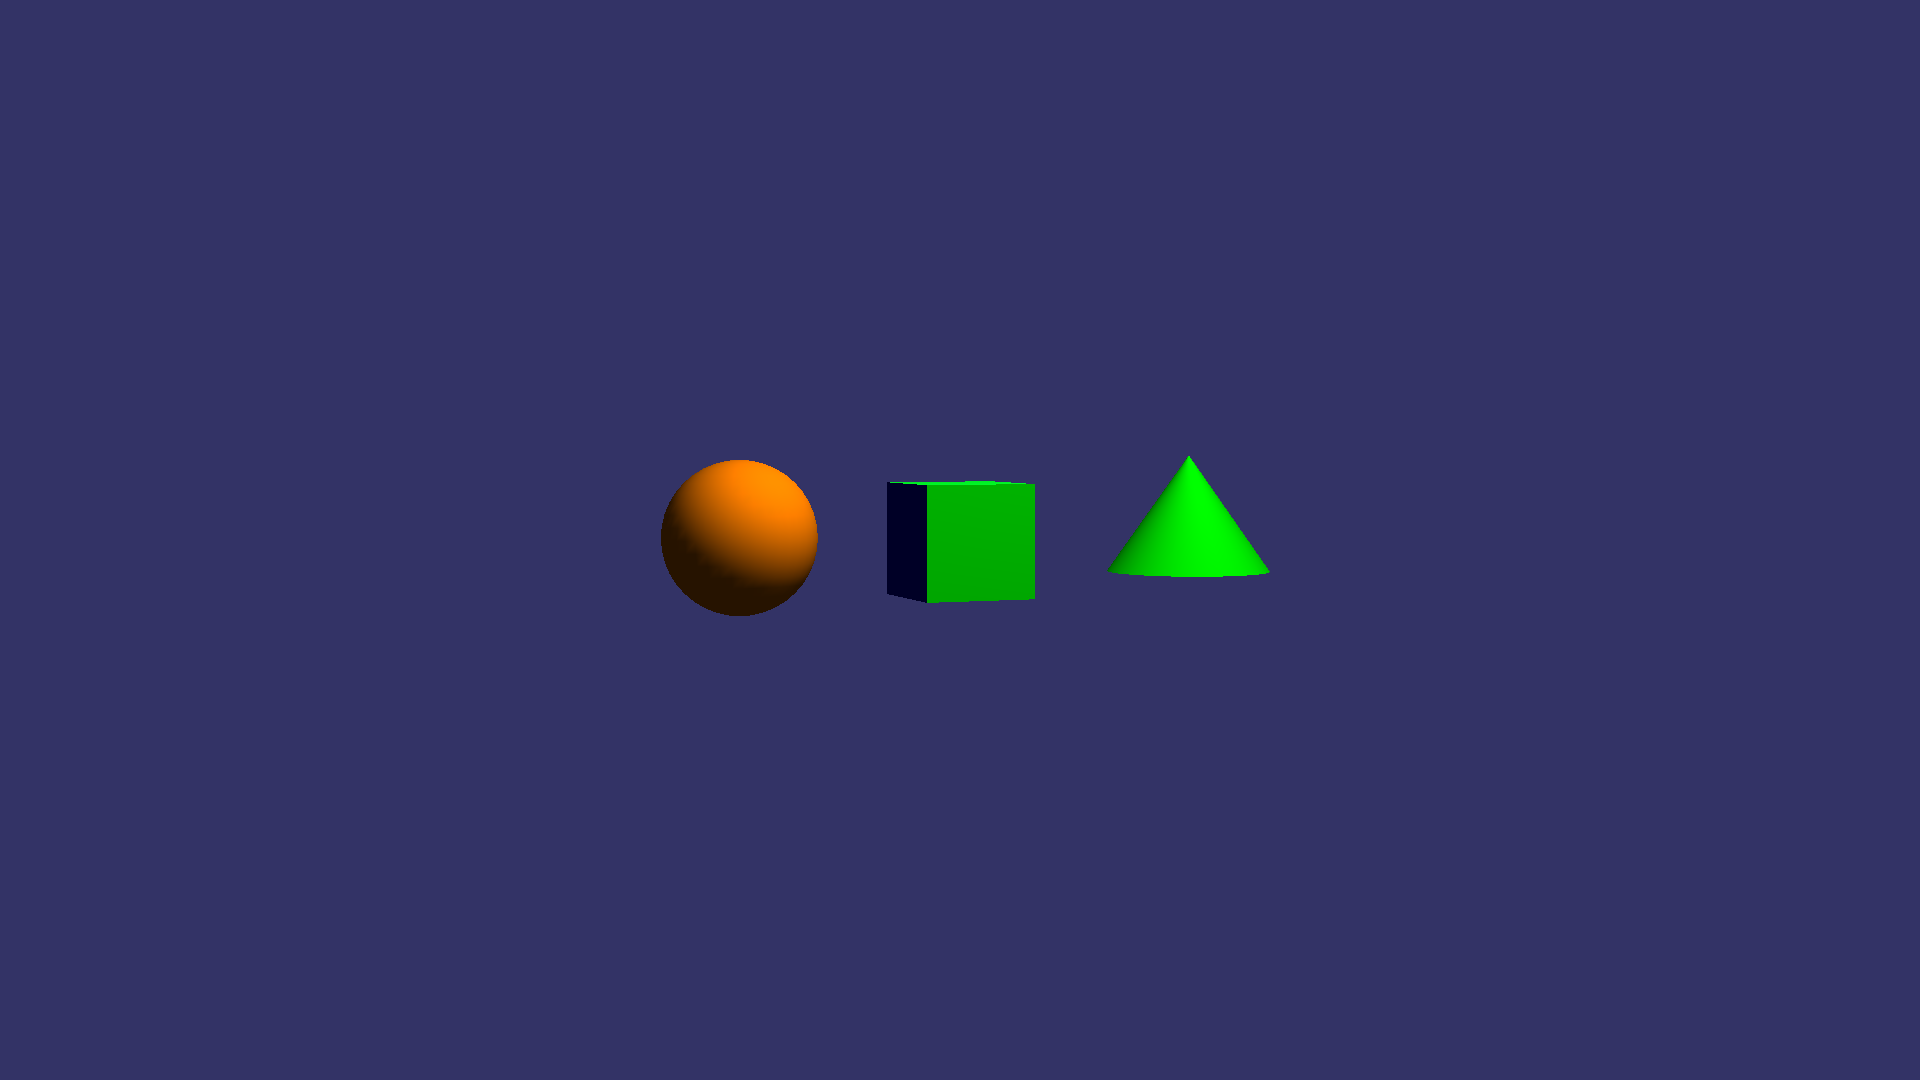
\includegraphics[width=\linewidth]{1osg}
\caption{Cámara 1 de OpenSceneGraph}
\label{fig:1osg}
\end{figure}

\begin{figure}[H]
\centering
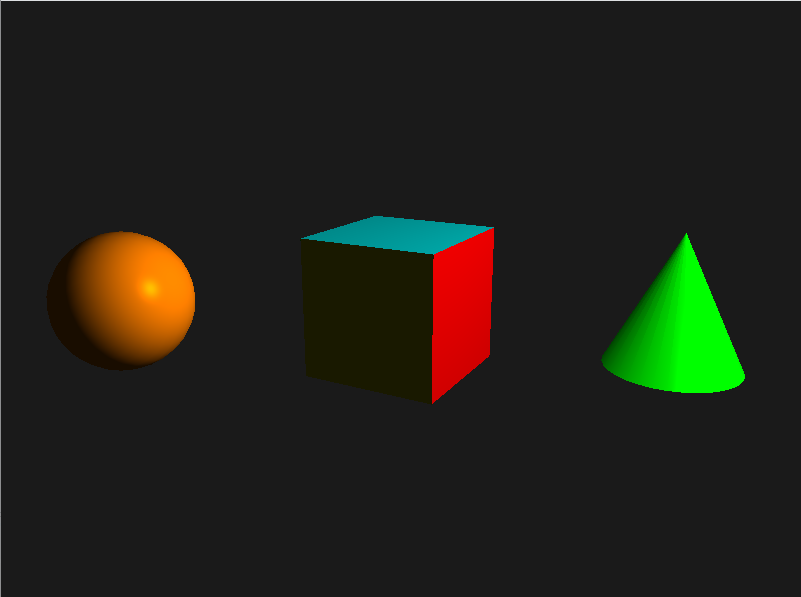
\includegraphics[width=\linewidth]{1gl}
\caption{Cámara 1 de OpenGL}
\label{fig:1gl}
\end{figure}

\begin{figure}[H]
\centering
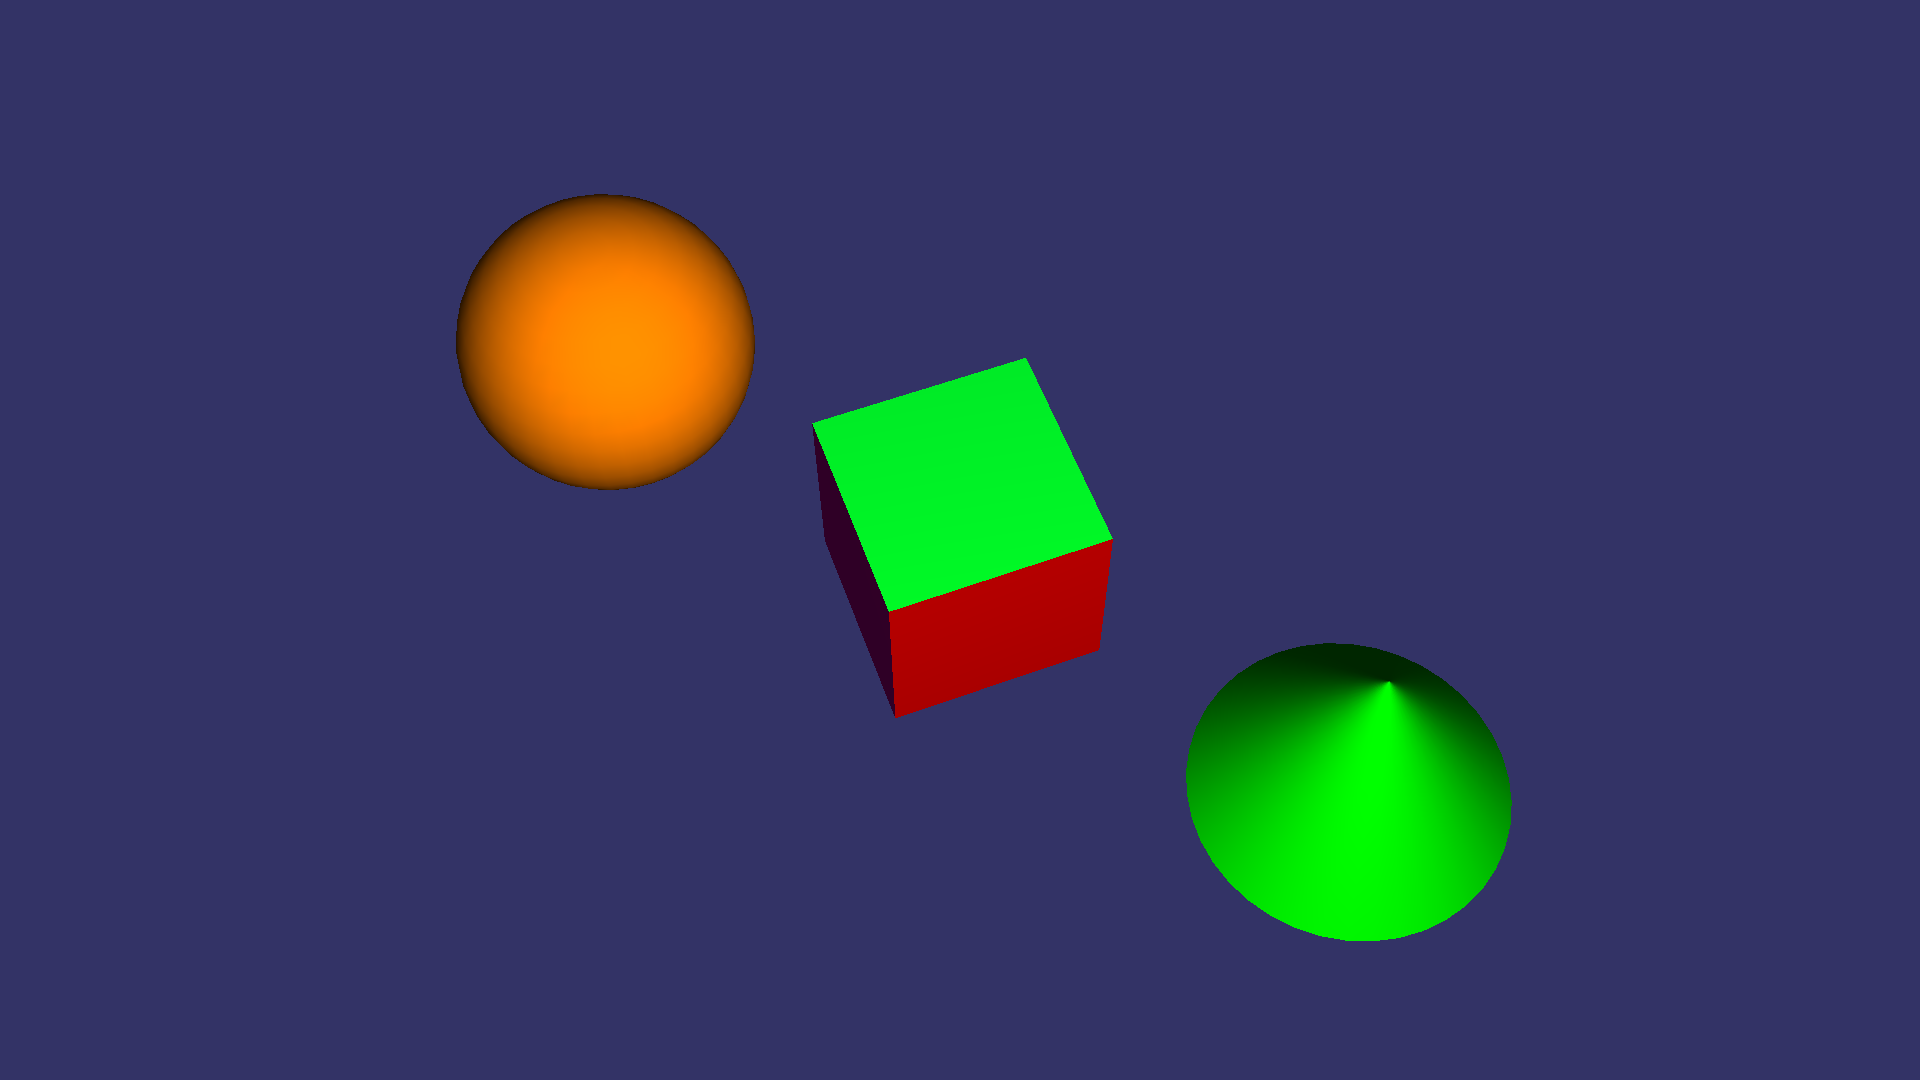
\includegraphics[width=\linewidth]{2osg}
\caption{Cámara 2 de OpenSceneGraph}
\label{fig:2osg}
\end{figure}

\begin{figure}[H]
\centering
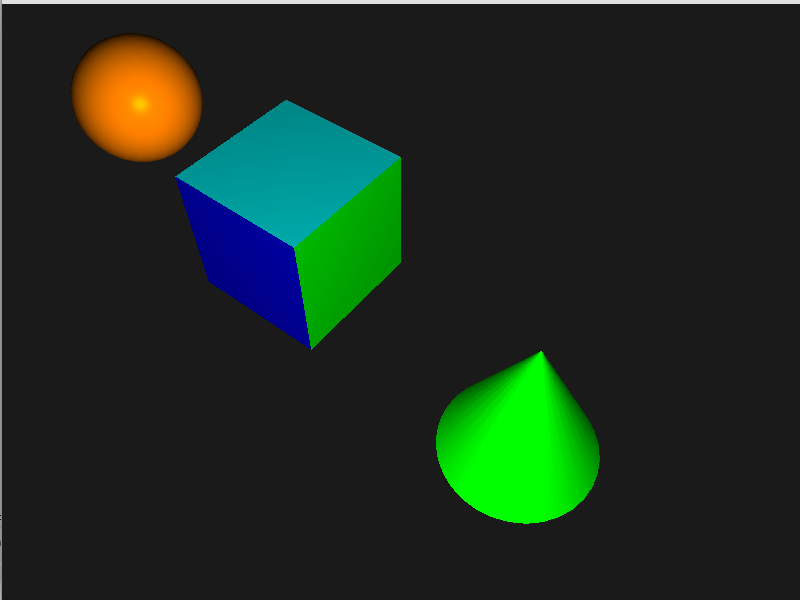
\includegraphics[width=\linewidth]{2gl}
\caption{Cámara 2 de OpenGL}
\label{fig:2gl}
\end{figure}

\begin{figure}[H]
\centering
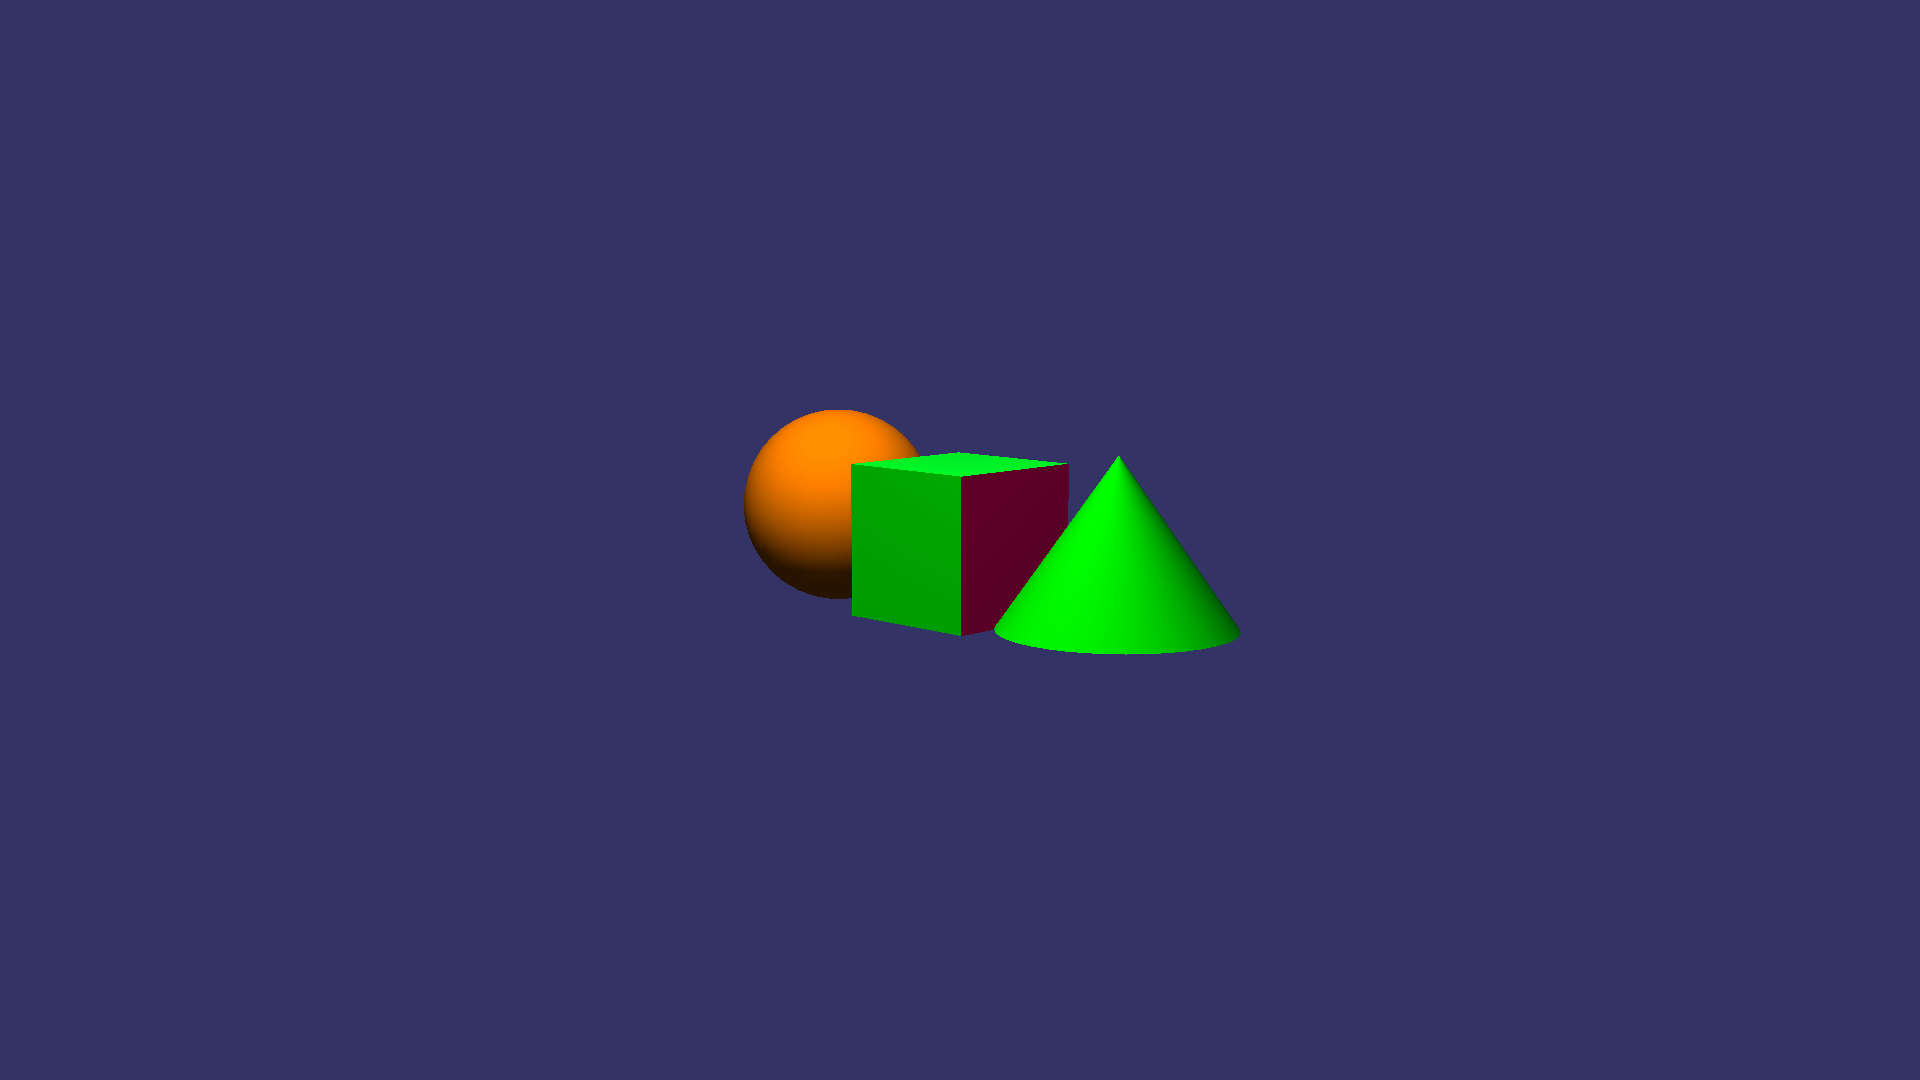
\includegraphics[width=\linewidth]{3osg}
\caption{Cámara 3 de OpenSceneGraph}
\label{fig:3osg}
\end{figure}

\begin{figure}[H]
\centering
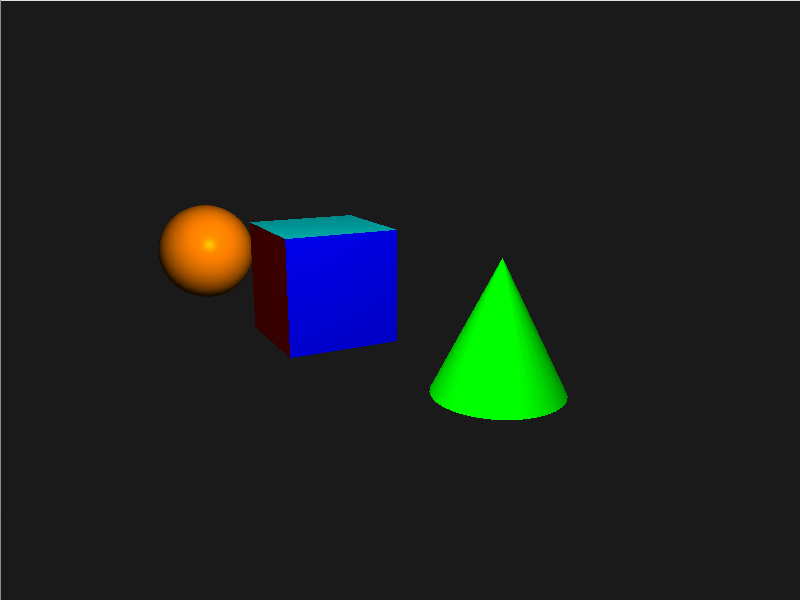
\includegraphics[width=\linewidth]{3gl}
\caption{Cámara 3 de OpenGL}
\label{fig:3gl}
\end{figure}

\end{document}

